\begin{frame}{Centralisé}
    \begin{block}{Le centralisé offre\dots}
        \begin{itemize}
            \item Diversité d'acteurs.
            \item Accessibilité.
            \item Multiples fonctionnalités.
        \end{itemize}
    \end{block}
    \pause
    \begin{block}{Mais\dots}
        \begin{itemize}
            \item Opacité des protocoles.
            \item Failles de sécurité.
            \item Collecte des données.
        \end{itemize}
    \end{block}
\end{frame}


\begin{frame}{Décantralisé}
    \begin{block}{Le décentralisé offre\dots\dots}
        \begin{itemize}
            \item Pas de tiers de confiance.
            \item Transparence.
            \item Fiabilité accrue.
        \end{itemize}
    \end{block}
    \pause
    \begin{block}{Mais\dots}
        \begin{itemize}
            \item Difficiles d'accès.
            \item Intérêt économique faible.
        \end{itemize}
    \end{block}
\end{frame}

\begin{frame}{Conclusion générale}
    \begin{itemize}
        \item Flou entre centralisé/décentralisé.
        \item Définition variable.
    \end{itemize}
\end{frame}

\begin{frame}
    \begin{figure}
        \begin{figure}
            \centering
            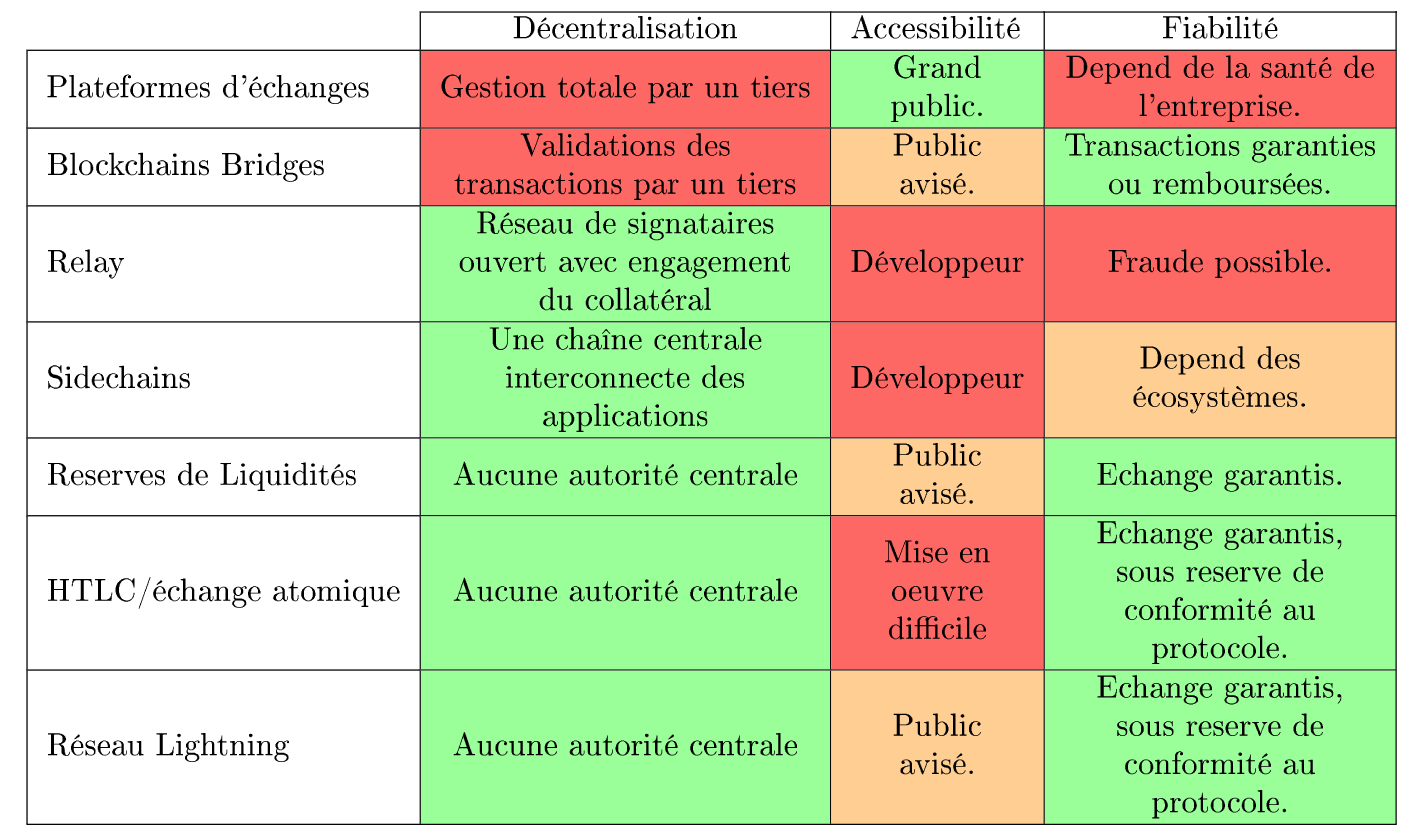
\includegraphics[scale = 0.2]{conclusion/tableau.png}
            \label{fig:recap}
            \caption{Tableau récapitulatif}
        \end{figure}
    \end{figure}
    
\end{frame}